\pagebreak
\section{Methods and Data: Forecasting Inflation with Machine Learning Models} \label{sec:methods}


\textbf{WHICH MODELS}

The general approach is to evaluate the model using an expanding window approach, i.e., in each month, the model will be trained on data available up to that month, which will in turn generate a forecast for the next month's inflation. 



\subsection{Models} \label{sec:methods_models}

\subsubsection{Random Walk Model}

The first benchmark model used is the Random Walk (RW) model, which assumes that the best predictor of tomorrow's value is today's value. Formally, the RW model for one-step-ahead forecasts is defined as:
\begin{equation}
    \widehat{y}_{t+h \mid t} = y_t
\end{equation}
for $h=1, \ldots, 12$, where $y_t$ is the last observed value at time $t$. For accumulated forecasts over $h$ months, the forecast is set as:
\begin{equation}
    \widehat{y}_{t+1:t+h \mid t} = y_{t-(h-1):t}
\end{equation}
where $y_{t-(h-1):t}$ represents the accumulated values of the target variable over the previous $h$ months. This model provides a baseline for assessing the predictive power of more complex models.

\subsubsection{Autoregressive Model}

The autoregressive (AR) model is a key benchmark in time series forecasting. It utilises historical values of the target variable to predict future values, assuming dependencies only on its own past values. Formally, the AR model is specified as:

\begin{equation}
    y_t = \beta_0 + \sum_{i=1}^{p} \beta_i y_{t-i} + \epsilon_t
\end{equation}

where:
\begin{itemize}
    \item $y_t$ represents the value of the target variable at time $t$,
    \item $p$ denotes the number of lags used, indicating the dependency of the forecast on $p$ past observations,
    \item $\beta_0, \beta_1, \ldots, \beta_p$ are coefficients estimated from the data, and
    \item $\epsilon_t$ is the error term, typically assumed to be independently and identically distributed with a mean of zero and constant variance.
\end{itemize}

The parameters are estimated using ordinary least squares (OLS), with the dependent variable being the current value of the target series, and the independent variables are the lagged values of the series. For a model with $n\_lags = p$, the predictor matrix $X$ is constructed as:

\begin{equation}
    X = \begin{bmatrix}
    y_{1} & y_{2} & \cdots & y_{p} \\
    y_{2} & y_{3} & \cdots & y_{p+1} \\
    \vdots & \vdots & \ddots & \vdots \\
    y_{T-p} & y_{T-p+1} & \cdots & y_{T-1}
    \end{bmatrix}
\end{equation}

where $T$ is the total number of observations in the training dataset.

Forecasts are generated by applying the estimated model to the lagged values present in the test dataset. This produces a series of one-step-ahead forecasts, facilitating direct comparison between forecasted and actual values.


\subsubsection{Random Forest Model}

Conceptually, a random forest comprises an ensemble of decision trees. Each decision tree in the ensemble serves to approximate the relationship between the target variable and the explanatory variables by partitioning the feature space into distinct subsets and producing a constant prediction for each subset. Specifically, in the context of regression—the focus of this discussion—the prediction within each subset is calculated as the mean of the target values encompassed by that subset. Conceptually, a decision tree may be characterised as a nonparametric regression model wherein the regression function linking the target to the features is estimated via a piecewise constant approach.

The segmentation of the feature space is executed recursively during the tree development phase. Initially, the tree is comprised of a single node—the root node—which encompasses the entire dataset. Within this node, the target prediction is made by averaging all observations of the target within the dataset. Subsequently, the dataset is recursively divided into increasingly smaller subsets, known as nodes. Each new node (child) originates from a subset of an existing node (parent), and the target prediction at each node is made by averaging the observations of the target within that node.

The divisions generating these nodes are driven by an optimisation process aimed at minimising a specific loss function, subject to constraints such as each node containing a minimum sample size. A commonly utilised loss function is the mean squared error of the prediction at each node, which equates to the variance of the target values within the node. This metric promotes the creation of nodes with homogeneous target values.

As the tree develops, progressively finer partitions of the feature space are established, enhancing the accuracy of the predictions. This refinement persists until a predetermined criterion is satisfied, such as each terminal node (leaf) comprising a minimum number of observations or the tree achieving a predetermined depth, measured by the number of nodes or recursive divisions from the root to the leaves.

Decision trees, however, are susceptible to overfitting. A sufficiently detailed tree could isolate individual target values within single leaves, thereby matching the training data's target values perfectly but failing to generalise effectively to novel, unseen data. Furthermore, decision trees demonstrate limited robustness to variations in input data, as minor modifications to the training data can lead to significantly different tree structures.

To mitigate these shortcomings, random forests employ multiple decision trees, each trained on distinct random subsets of the training data (a technique known as sample bagging) and utilising varied random subsets of features (feature bagging). The final predictions of a random forest are derived by averaging the predictions from each tree within the ensemble. This approach of sample and feature bagging diminishes the correlation among the trees' predictions, thereby enhancing the robustness of the ensemble and reducing its susceptibility to overfitting.

In the context of macroeconomic forecasting, random forests are particularly valuable for several reasons. Random forests provide an intrinsic mechanism to evaluate the importance of various predictors in forecasting economic conditions. This feature is crucial in selecting key economic indicators that most significantly impact the macroeconomic variables being forecasted. The out-of-bag error estimation also offers an efficient method for validating the model’s performance without the need for a separate validation dataset. This is especially useful in economics where the availability of data can be limited, and traditional cross-validation might lead to overfitting. Furthermore, given the complexity and noise inherent in economic data, random forests’ robustness to overfitting and ability to handle large feature spaces make them ideal for capturing complex nonlinear relationships that are typical in macroeconomic interactions.



\begin{figure}[h] 
\vspace{5mm}
\centering 
\begin{forest}
  for tree={l sep=1.5em, s sep=1.5em, anchor=center, inner sep=0.3em, fill=blue!50, circle, where level=2{no edge}{}}
  [
  Training Data, node box
  [Sample and feature bagging, node box, alias=bagging, above=3em
  [,red!70,alias=a1[[,alias=a2][]][,red!70,edge label={node[above=0.5ex,red arrow]{}}[[][]][,red!70,edge label={node[above=0.5ex,red arrow]{}}[,red!70,edge label={node[below=0.5ex,red arrow]{}}][,alias=a3]]]]
  [,red!70,alias=b1[,red!70,edge label={node[below=0.5ex,red arrow]{}}[[,alias=b2][]][,red!70,edge label={node[above=0.5ex,red arrow]{}}]][[][[][,alias=b3]]]]
  [~~$\dots$~,scale=1.5,no edge,fill=none,yshift=-2em]
  [,red!70,alias=c1[[,alias=c2][]][,red!70,edge label={node[above=0.5ex,red arrow]{}}[,red!70,edge label={node[above=0.5ex,red arrow]{}}[,alias=c3][,red!70,edge label={node[above=0.5ex,red arrow]{}}]][,alias=c4]]]]
  ]
  \node[tree box, fit=(a1)(a2)(a3)](t1){};
  \node[tree box, fit=(b1)(b2)(b3)](t2){};
  \node[tree box, fit=(c1)(c2)(c3)(c4)](tn){};
  \node[below right=0.5em, inner sep=0pt] at (t1.north west) {Tree 1};
  \node[below right=0.5em, inner sep=0pt] at (t2.north west) {Tree 2};
  \node[below right=0.5em, inner sep=0pt] at (tn.north west) {Tree $n$};
  \path (t1.south west)--(tn.south east) node[midway,below=3em, node box] (mean) {Mean in regression or majority vote in classification};
  \node[below=2em of mean, node box] (pred) {Prediction};
  \draw[black arrow={4mm}{3mm}] (bagging) -- (t1.north);
  \draw[black arrow] (bagging) -- (t2.north);
  \draw[black arrow={4mm}{3mm}] (bagging) -- (tn.north);
  \draw[black arrow={4mm}{4mm}] (t1.south) -- (mean);
  \draw[black arrow] (t2.south) -- (mean);
  \draw[black arrow={4mm}{4mm}] (tn.south) -- (mean);
  \draw[black arrow] (mean) -- (pred);
\end{forest}
\caption[Random forest diagram]{A visual representation of a random forest model showing sample and feature bagging, decision trees, and the averaging process.\footnotemark}
\end{figure}

\footnotetext{This diagram is based on conceptual material from "Random Forests and Decision Trees from Scratch in Python" by Towards Data Science, available at \url{https://towardsdatascience.com/random-forests-and-decision-trees-from-scratch-in-python-3e4fa5ae4249}. Adaptations and modifications were made to the TikZ code originally found on TeX StackExchange at \url{https://tex.stackexchange.com/questions/503883/illustrating-the-random-forest-algorithm-in-tikz}.}


This paper follows the random forest method set out in \textcite{Medeiros2021ForecastingMethods}. The model draws on the original ideas proposed in \textcite{Breiman2001RandomForests}. This approach constructs a multitude of regression trees on bootstrapped subsets of the data, each tree making local predictions by recursively partitioning the covariate space. A regression tree approximates an unknown nonlinear function by dividing the covariate space into distinct regions, within which the response variable is predicted with a constant estimated from the data. For instance, given explanatory variables $X_1$ and $X_2$, the partition might first split on $X_1=s_1$, and subsequent splits on $X_2=s_2$ and $X_1=s_3$, leading to several distinct regions. Within each region $R_k$, the model predicts the dependent variable $Y$ with a constant value $c_k$, calculated as the average of $Y$ values within that region. Each tree is thus a series of binary decisions leading to terminal nodes, where each node corresponds to a region in the input space. The Random Forest model aggregates several such trees to form a robust predictor. Each tree is built on a different bootstrap sample of the dataset, allowing for variations in the structure and splits of each tree. This process helps in reducing the variance of the model without substantially increasing the bias.

Formally, the model for a given dependent variable $\pi_{t+h}$ and a vector of predictors $\boldsymbol{x}_t$ can be described by:
$$
\widehat{\pi}_{t+h} = \frac{1}{B} \sum_{b=1}^B \left[ \sum_{k=1}^{K_b} \widehat{c}_{k, b} \mathbf{I}_{k, b}\left(\boldsymbol{x}_t ; \widehat{\boldsymbol{\theta}}_{k, b}\right) \right]
$$
where:
\begin{itemize}
    \item $B$ is the number of bootstrap samples,
    \item $K_b$ is the number of terminal nodes (regions) in the $b$-th tree,
    \item $\widehat{c}_{k, b}$ is the predicted value for region $k$ in bootstrap sample $b$,
    \item $\mathbf{I}_{k, b}$ is an indicator function that is 1 if $\boldsymbol{x}_t$ falls into region $k$ of the $b$-th tree and 0 otherwise, and
    \item $\widehat{\boldsymbol{\theta}}_{k, b}$ are the parameters defining the splits that lead to the $k$-th region in the $b$-th sample.
\end{itemize}

The dataset is prepared by including lagged values of the target variable and applying principal components analysis to reduce dimensionality, forming a comprehensive set of predictors. The Random Forest model utilizes these predictors to generate forecasts for each observation in the test dataset. The final forecast for $\pi_{t+h}$ is the average of the forecasts from all trees in the forest, applied to the original data. The model's effectiveness is assessed by comparing its forecast accuracy against actual observed values, using metrics such as the root mean squared error (RMSE), mean absolute error (MAE), and median absolute deviation (MAD). This methodology provides a powerful approach to forecasting, capable of capturing complex nonlinear relationships in the data while maintaining robustness through averaging multiple predictions.


% The Random Forest model is specified with a set of hyperparameters that are optimised for time series forecasting. The hyperparameters include:
% \begin{itemize}
%     \item Number of trees (\texttt{n\_estimators}).
%     \item Maximum number of features considered for splitting a node (\texttt{max\_features}).
%     \item Minimum number of samples required at a leaf node (\texttt{min\_samples\_leaf}).
%     \item Control for the random number generation to ensure reproducibility (\texttt{random\_state}).
% \end{itemize}

% The Random Forest model is trained on a dataset comprising historical values of the target variable and potentially other explanatory variables derived through principal components analysis (PCA) to reduce dimensionality. The training data includes:
% \begin{equation}
%     \textbf{X} = [\text{lagged values of target}, \text{principal components}]
% \end{equation}
% and the model is tasked to predict:
% \begin{equation}
%     y_t = \text{value of target variable at time } t.
% \end{equation}

% Forecasts are generated for each vintage of the dataset by applying the trained Random Forest model to the test data, which includes lagged values of the target variable and principal components up to the current vintage. The output is a series of one-month-ahead forecasts.

% The forecasting performance of the Random Forest model is evaluated against actual values by calculating root mean squared error (RMSE), mean absolute error (MAE), and median absolute deviation (MAD) for the forecasted versus actual values. Comparative analyses are also performed against other models, including an autoregressive (AR) model and a random walk (RW) model, to assess the relative performance:

% \begin{equation}
%     \text{Error Metric Ratio} = \frac{\text{Error Metric of RF Model}}{\text{Error Metric of Comparison Model}} - 1
% \end{equation}

\subsubsection*{Discussion of Random Forest Model}

The performance of the Random Forest model critically depends on the appropriate tuning of its hyperparameters, which are selected to optimise the model's accuracy and computational efficiency while ensuring its robustness to overfitting. These parameters are set based on empirical evidence and theoretical considerations, aimed at achieving optimal predictive performance.

\subsubsection*{Number of Trees}

The number of trees, specified by the hyperparameter \texttt{n\_estimators}, is set to 500. This choice is designed to provide a high level of accuracy while also ensuring that the model's performance stabilises, as increasing the number of trees beyond this point typically yields diminishing returns in terms of error reduction \autocite{Medeiros2021ForecastingMethods}. A larger number of trees enhances the ensemble's ability to generalise, thereby mitigating variance without unduly increasing bias. Choosing a smaller number of trees could lead to increased model variance and potentially underfitting, while an excessively large number might not only waste computational resources but also not yield proportional gains in performance.

\subsubsection*{Maximum Features per Split}

The hyperparameter \texttt{max\_features} is set to one-third of the total number of features available. This parameter controls the number of features considered when determining the best split at each node of the trees. By restricting the number of features, this setting helps in maintaining a diversity among the trees, preventing the model from fitting too closely to the training data. It strikes a balance between exploring new attribute combinations and retaining prediction accuracy, which is crucial in handling complex economic data structures. Setting \texttt{max\_features} too high could increase the correlation between the trees, reducing the benefit of bagging by making the ensemble too similar to a single decision tree, whereas setting it too low might not capture sufficient information and could increase bias.

\subsubsection*{Minimum Samples per Leaf}

Set at a minimum of five, the \texttt{min\_samples\_leaf} parameter ensures that each terminal node (leaf) in the tree structures contains no fewer than five data points. This setting helps in preventing the trees from growing overly complex and sensitive to specific samples in the training data, thus enhancing the model's generalisability and robustness against noise and outliers commonly present in economic time series data. A lower threshold might allow the model to capture more detailed information but at the risk of overfitting, while a higher threshold might simplify the model excessively, potentially ignoring valuable information in smaller subsets of data.

\subsubsection{Lasso Model}





\subsection{Data: FRED-MD} \label{sec:methods_data}

FRED-MD is a large macroeconomic database designed for the empirical analysis of “big data” \autocite{McCracken2016FRED-MD:Research}. The dataset has become a popular resource for modelling US macro variables, due to the number of variables, the length of the time series and the regularity of updates.

The dataset is of monthly observations, updated on a monthly basis. Each monthly release is referred to as a vintage. A different CSV file is released for each month. The data is publicly accessible.\footnote{The latest vintage, as of the time of publication, is available at: \url{https://files.stlouisfed.org/files/htdocs/fred-md/monthly/2024-04.csv}. The historical vintages can be accessed directly at \url{https://s3.amazonaws.com/files.research.stlouisfed.org/fred-md/Historical_FRED-MD.zip}
} The sample spans from March, 1959 to the present, providing us with a relatively rich data set of macroeconomic time series with $x = 127$ variables and $t = 780$ observations. These variables are grouped under eight headings of macroeconomic indicators: output and income, labour market, consumption and orders, orders and inventory, money and credit, interest rates and exchange rates, prices, and stock market.

As the focus of this paper in inflation forecasting, the dependent variable of interest throughout the analysis is \texttt{CPIAUCSL}. I use the data from January 2015 to January 2024 for the analysis throughout the paper.

A full list of the variables available in FRED-MD is included in the Appendix, at \S \ref{sec:appendix_var}. The data is not stationary by default but the first row of the CSV file contains the relevant transformations needed to prepare the data. The codes are as follows:

\begin{enumerate}
    \item no transformation,
    \item first order difference,
    \item second order difference,
    \item logarithm,
    \item first order logarithmic difference,
    \item second order logarithmic difference, and
    \item percentage change.
\end{enumerate}

The dataset is divided into two subsets: training data (\texttt{train\_data}) and test data (\texttt{test\_data}). The training data is used to estimate the parameters of the model, while the test data is used to evaluate the model's forecasting ability.

\begin{figure}[H]
    \centering
    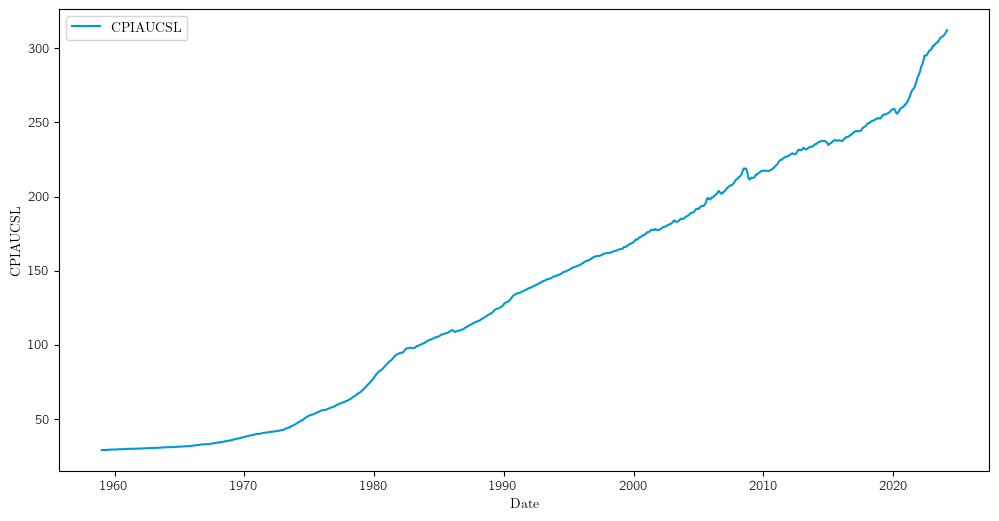
\includegraphics[width=1\linewidth]{figures/cpi.png}
    \vspace{-30pt}
    \caption{CPI, all items, 1960-2024.}
    \label{fig:cpi} 
\end{figure}
